\documentclass[aspectratio=169]{beamer}
\input{../utils/beamerpreamble.tex}

\subtitle[Statistical Indicators]{Topic 02 - Descriptive Experiments, Point and Interval Indicators}

\begin{document}

% TODO: Move 10_Descriptive_Experiment to lecture 1, and move some of the content from lecture 1 to later lectures.

\begin{frame}
  \maketitle

  \vfill

  \hfill \tiny{Version 2024}
\end{frame}

\begin{frame}[t]{Outline}
  Topics for today:
  \begin{itemize}
    \item \structure{Descriptive Experiments}: We walk through a few simple experiments, and what points we need to pay attention to when designing the experiment.
    \item \structure{Point and Interval Indicators}: We formalize how we talk about the results of descriptive experiments, and how we measure experimental error.
  \end{itemize}

  \bigskip
  A few keywords for this lecture:
  \begin{itemize}
    \item Experimental Question
    \item Response Variable and Control Variable
    \item Models, Random Variables, and Distributions
    \item Mean and Standard deviation
    \item Estimator and Error
  \end{itemize}
  
\end{frame}

\section{Designing a Simple Experiment}

\begin{frame}[t]{Section I: A simple experiment}
    In this section, we discuss the design of simple experiments.
    \bigskip

    We talk about:
    \begin{itemize}
        \item Defining the experimental question;
        \item Defining the variables and condition of the experiment;
        \item Noise in Experiment;
    \end{itemize}    
\end{frame}

\subsection{Do you even lift?}

\begin{frame}[t]{Do you even lift, bro?}
    Let's imagine a simple experiment, where you want to measure how much weight you are capable of lifting.
    \bigskip 

    How would you perform this experiment?    

    \vfill

    \hfill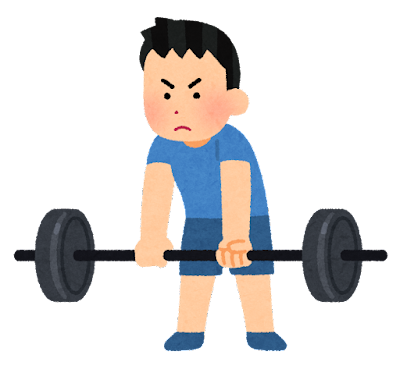
\includegraphics[width=0.3\textwidth]{img/irasutoya_lift.png}
    \ppagenote{Lifting image from \url{https://www.irasutoya.com}}
\end{frame}

\begin{frame}[t]{Desigining an experiment}
    There are many questions that we should consider when we design this experiment. Here are a few examples:
    \begin{itemize}
        \item What kind of weight are we lifting? How do we measure the weight?
        \item What movement is performed? Deadlift? Benchpress? Weight backpack?
        \item What is the environment for the experiment? Tiredness? Physical preparation?        
        \item Are there any sources of variation that could affect the result?
    \end{itemize}\bigskip

    If you stop to think about it, you can probably think of many other questions. \structure{When do you stop?}
\end{frame}

\subsection{Clarifying the experiment}

\begin{frame}[t]{First things first: Specify the experiment question!}

    To help answer the design questions, the most important thing we can do is to {\bf specify the experimental question of interest}.\bigskip

    What we want to know has a very large influence in how we design the experiment:
    \begin{enumerate}
        \item \structure{We want to know if we have a chance to win a weight lifting competition.} In this case, we want our experiment to be as similar as the competition as possible. Our objective is to measure the maximum weight we could lift.
        \item \structure{We want to decide a good weight to use for hypertrophy training}. In this case, we need to define the number of repetitions, and find out the maximum weight we can lift for those repetitions, in a training context (other exercises, etc).
        \item \alert{We want to know how heavy our emergency kit should be}. In this case, we want to find out how much weight we can carry in a backpack, while being able to quickly leave a building, and possibly walking a long distance.
    \end{enumerate}
\end{frame}

\begin{frame}[t]{A good experiment has a good question}
    Note how for the same question (how much weight can you lift) we can imagine completely different experiments.\bigskip

    It is {\bf extremely important} to clarify what you want to know, and why, when desigining your experiment.\bigskip 

    The answers to experiment design questions will be easier to find if you know what you are looking for. \alert{On the other hand, doing an experiment without a clear objective or question will cause you to ignore important parts of the design}.\bigskip 

    {\bf TL;DR: Do experiments about things that you care about!}
\end{frame}

\begin{frame}[t]{Observed Variables and Experiment Conditions}

    One way to organize a simple experiment is to define the \structure{observed variable} and the \structure{experiment conditions}.\bigskip
    
    \begin{itemize}
        \item The \structure{observed variable} is the data that we collect and analyze from the experiment. 
        
        \item The \structure{experiment conditions} are the environment in which the experiment takes place.
    \end{itemize}\bigskip

    When defining the conditions, it may be useful to clarify the elements of the experiment that you {\bf can control} and that you \alert{cannot control}.
\end{frame}

\begin{frame}[t]{Experiment Design Example 1}{Can you even lift?}
    \begin{itemize}
        \item \structure{Experimental Question:} What weight should I use for a repetition exercise?
        \item \structure{Observed Variable:} Raise amount of weight until failure;
        \item \structure{Experiment Conditions}: Correct form; Usual time for exercise; Stretching; Define failure as not being able to complete the exercise correctly; Raise the weight by 2.5kgs after each success.
    \end{itemize}\medskip

    Note that you can and should expand on these points!
    \hfill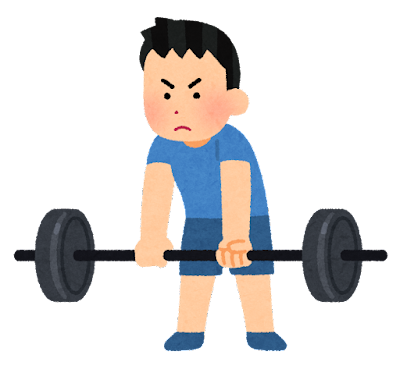
\includegraphics[width=0.2\textwidth]{img/irasutoya_lift.png}

\end{frame}

\begin{frame}[t]{Experiment Design Example 2}{Bycicle Ride}
    \begin{itemize}
        \item \structure{Experimental Question}: What time should I leave to arrive in time for class?
        \item \structure{Observed Variable}: The minimum bicycle time from dormitory to class (or the maximum time?)
        \item \structure{Experiment Conditions}: Bicycle maintenance? Good weather or bad weather? What time should you do the experiment? What do you use to measure the time?
    \end{itemize}\medskip

    The goal of the experiment influences the measures and conditions!
    \hfill
\includegraphics[width=0.2\textwidth]{img/irasutoya_bicycle.png}
    \ppagenote{Cycling image from \url{https://www.irasutoya.com}}
\end{frame}

\begin{frame}[t]{Experiment Design Example 3}{Algorithm Accuracy}
    \begin{itemize}
        \item \structure{Experimental Question}: What is the accuracy of a machine learning algorithm?
        \item \structure{Observed Variable}: The testing accuracy of the algorithm on (a single dataset? a group of datasets?)
        \item \structure{Experiment Conditions}: Are the datasets representative of the problem? What is the effect of the random seed? What should be the hyper parameters? What is the computer and library versions? 
    \end{itemize}

    \hfill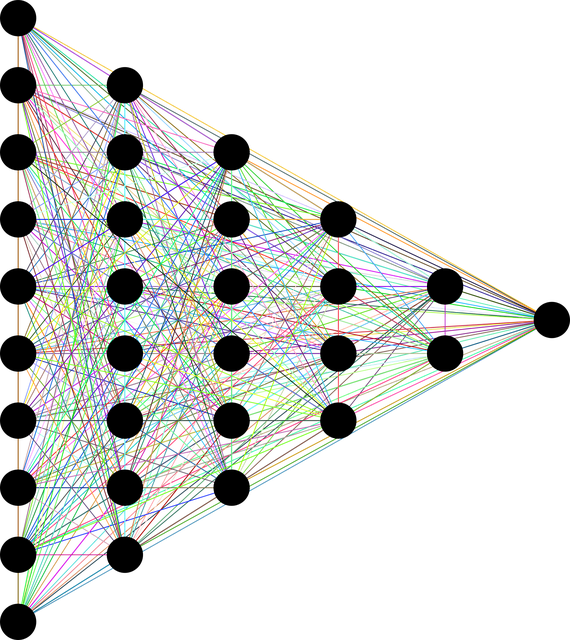
\includegraphics[width=0.15\textwidth]{../img/pixabay_neuralnetwork_gordonjohnson.png}
    \ppagenote{Neural Network image from pixabay}
\end{frame}

%%%%%%%%%%%%%%%%%%%%%%%%%%%%%%%
\subsection{Experiment and Noise}

\begin{frame}[t]{Experiments and Noise -- a question for you:}
    Imagine you do the bicycle experiment two times. 
    
    \begin{itemize}
        \item The first time, you complete the course in 30 minutes. 
        \item The second time, you complete the course in 40 minutes.
    \end{itemize}\bigskip

    What does this mean for your experiment?\bigskip    

    And more importantly: When should you leave the dormitory to arrive at the class in time?

    \hfill
\includegraphics[width=0.2\textwidth]{img/irasutoya_bicycle.png}
\end{frame}

\begin{frame}[t]{What is experimental noise?}
    Noise (or sometimes error) is when you get different results when repeating the same experiment.\medskip 

    How you handle the noise depends on the objective of your experiment:
    \begin{itemize}
        \item Lifting: You use the average value for your exercise;
        \item Results of an English Exam: You report the highest value;
        \item Bridge Engineering: You use the lowest value as safety;
    \end{itemize}
\end{frame}

\begin{frame}[t]{Why do we have noise?}
    \begin{itemize}
        \item There are many conditions that can influence the result of our experiment;
        \item Some conditions we cannot control, some we don't even know;
        \item Experiment design usually include a "noise factor" or "error factor" to consider all the unknowns;
        \item \alert{It is possible to measure and quantify the error!}
    \end{itemize}   
\end{frame}


\subsection{A few words on experiment design}

\begin{frame}[t]{Experiment Design is not easy!}
    Pay attention how the choices you make for observed variable and experiment condition will affect the answer to your experimental question!\bigskip

    The design of an experiment is an \structure{iteractive} process. A well defined question will help you choose variables and conditions. And as you consider the variables and conditions, you will reflect on your question again.\bigskip

    Keep notes of what decisions you make for your experiments, and why. Future you will be grateful!\bigskip 

    \begin{block}{}
    Keep the focus on the {\bf why} of the experiment. Keep {\bf curiosity and honesty}.
    \end{block}
\end{frame}

\begin{frame}{Break}
    Break time. How can you use these topics on your experiments?
\end{frame}



% TODO
%\section{Variables, Model and Noise}

\begin{frame}{Variables, Model and Noise}{What we will learn in this section}


    
\end{frame}
%\section{Point and Interval Estimators}

\begin{frame}{Point and Interval Estimators}{What we will learn in this section}
    
\end{frame}

% Old Slides
\input{old_indicators.tex}

%% Recommended Reading %%
\begin{frame}{Recommended Reading}
  \begin{itemize}
    \item \emph{D.W. Stockburger}, The Sampling Distribution. In: Introductory Statistics: Concepts, Models, and Applications -
    \url{http://psychstat3.missouristate.edu/Documents/IntroBook3/sbk17.htm}
    \item \emph{J.G. Ramírez}, Statistical Intervals: Confidence, Prediction, Enclosure: \url{https://git.io/v5ZFh}
    \item Crash Course Statistics Playlist, in particular videos \#3 to \#7: \url{https://www.youtube.com/playlist?list=PL8dPuuaLjXtNM_Y-bUAhblSAdWRnmBUcr}
  \end{itemize}
\end{frame}

%%%%%%%%%%%%%%%%%%%%%%%%%%%%%%%%%%%%%%%%%%%%%%%%%%%%
\input{../utils/lastslide.tex}
\end{document}
